\chapter{Análisis y Diseño}
En este capítulo se presenta el modelo del dominio, el modelo conceptual\footnote{Se incluye un modelo conceptual por paquetes en el Apéndice \ref{appendix:paquetes}} y el modelo físico en su versión final. Posteriormente se describe la estructura y se desarrolla cada casos de uso de acuerdo a ICONIX.

\pagebreak
\section{Modelo del Dominio}
    \begin{figure}[H]
        \centering
        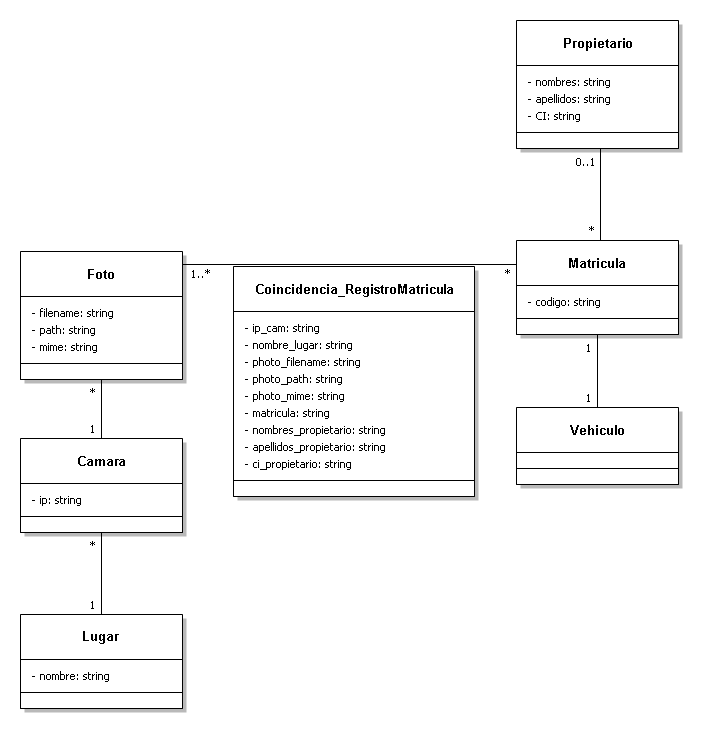
\includegraphics[width=.9\textwidth]{DOM2}
        \caption{Modelo del Dominio}
        \label{fig:DOM}
    \end{figure}
\section{Modelo Conceptual}

 \begin{figure}[H]
        \centering
        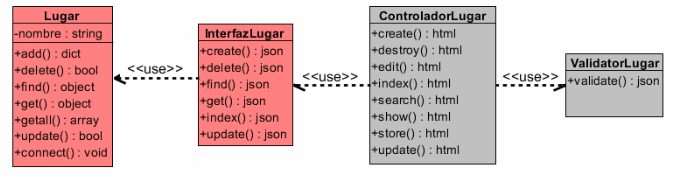
\includegraphics[width=.9\textwidth]{CLASS-lugar}
        \caption{Diagrama de Clases - Lugar}
        \label{fig:class-lugar}
    \end{figure}
 \begin{figure}[H]
        \centering
        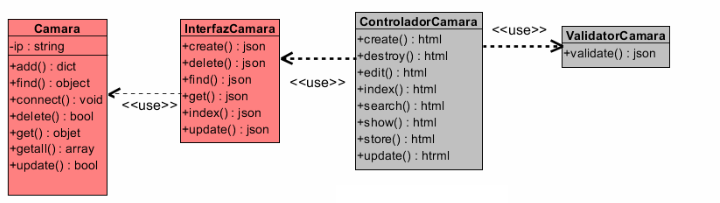
\includegraphics[width=.9\textwidth]{CLASS-cam}
        \caption{Diagrama de Clases - Cámara}
        \label{fig:class-camara}
    \end{figure}
 \begin{figure}[H]
        \centering
        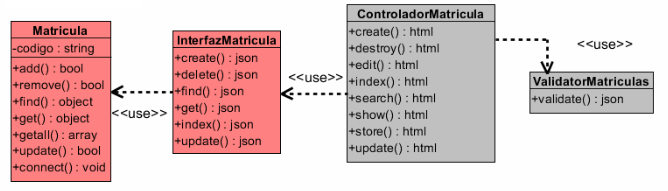
\includegraphics[width=.9\textwidth]{CLASS-matri}
        \caption{Diagrama de Clases - Matrícula}
        \label{fig:class-matricula}
    \end{figure}

 \begin{figure}[H]
        \centering
        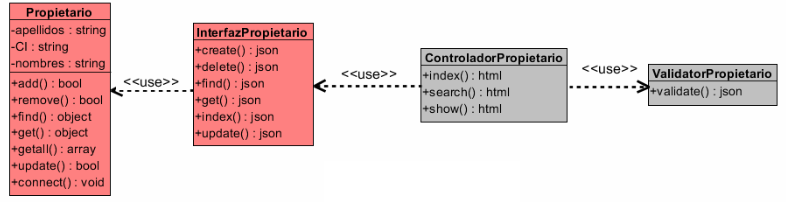
\includegraphics[width=.9\textwidth]{CLASS-prop}
        \caption{Diagrama de Clases - Propietario}
        \label{fig:class-propietario}
    \end{figure}
    
     \begin{figure}[H]
        \centering
        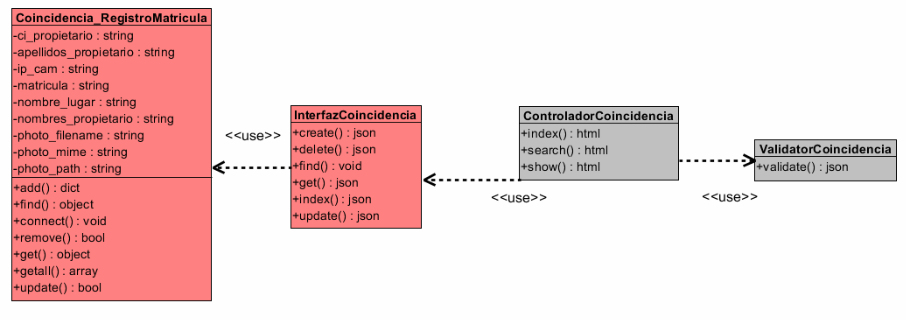
\includegraphics[width=.9\textwidth]{CLASS-coin}
        \caption{Diagrama de Clases - Coincidencia}
        \label{fig:class-coincidencia}
    \end{figure}

 \begin{figure}[H]
        \centering
        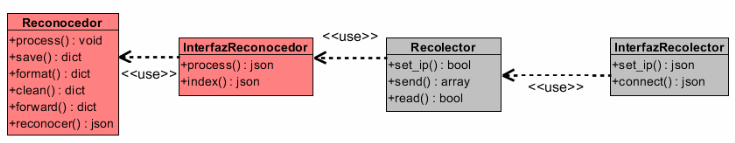
\includegraphics[width=.9\textwidth]{CLASS-reco}
        \caption{Diagrama de Clases - Reconocedor \& Recolector}
        \label{fig:class-reconocedor}
    \end{figure}


 \begin{figure}[H]
        \centering
        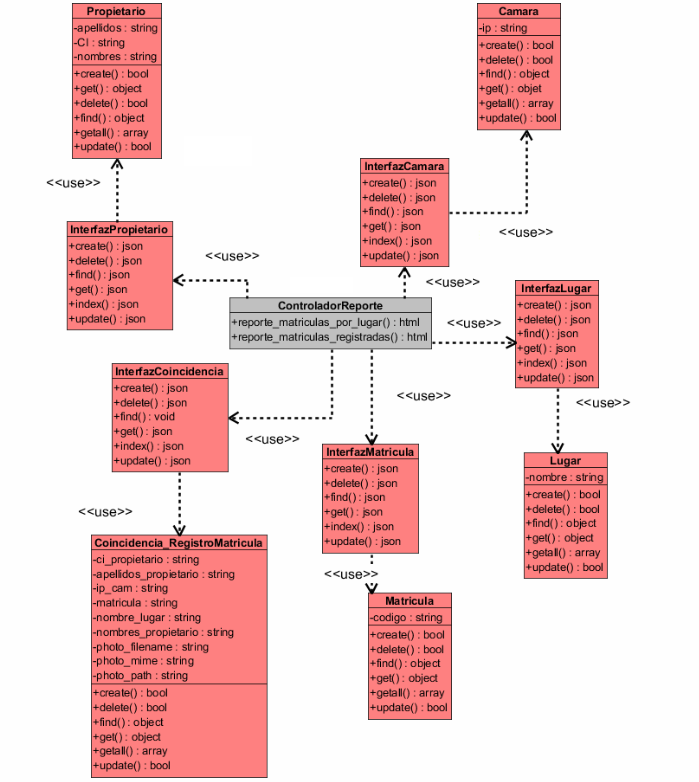
\includegraphics[width=.9\textwidth]{CLASS-repo}
        \caption{Modelo Conceptual - Controlador de Reportes}
        \label{fig:CLASS-repo}
    \end{figure}
    
% \eject \pdfpagewidth=420mm \pdfpageheight=297mm
%     \begin{figure}[H]
%         \centering
%         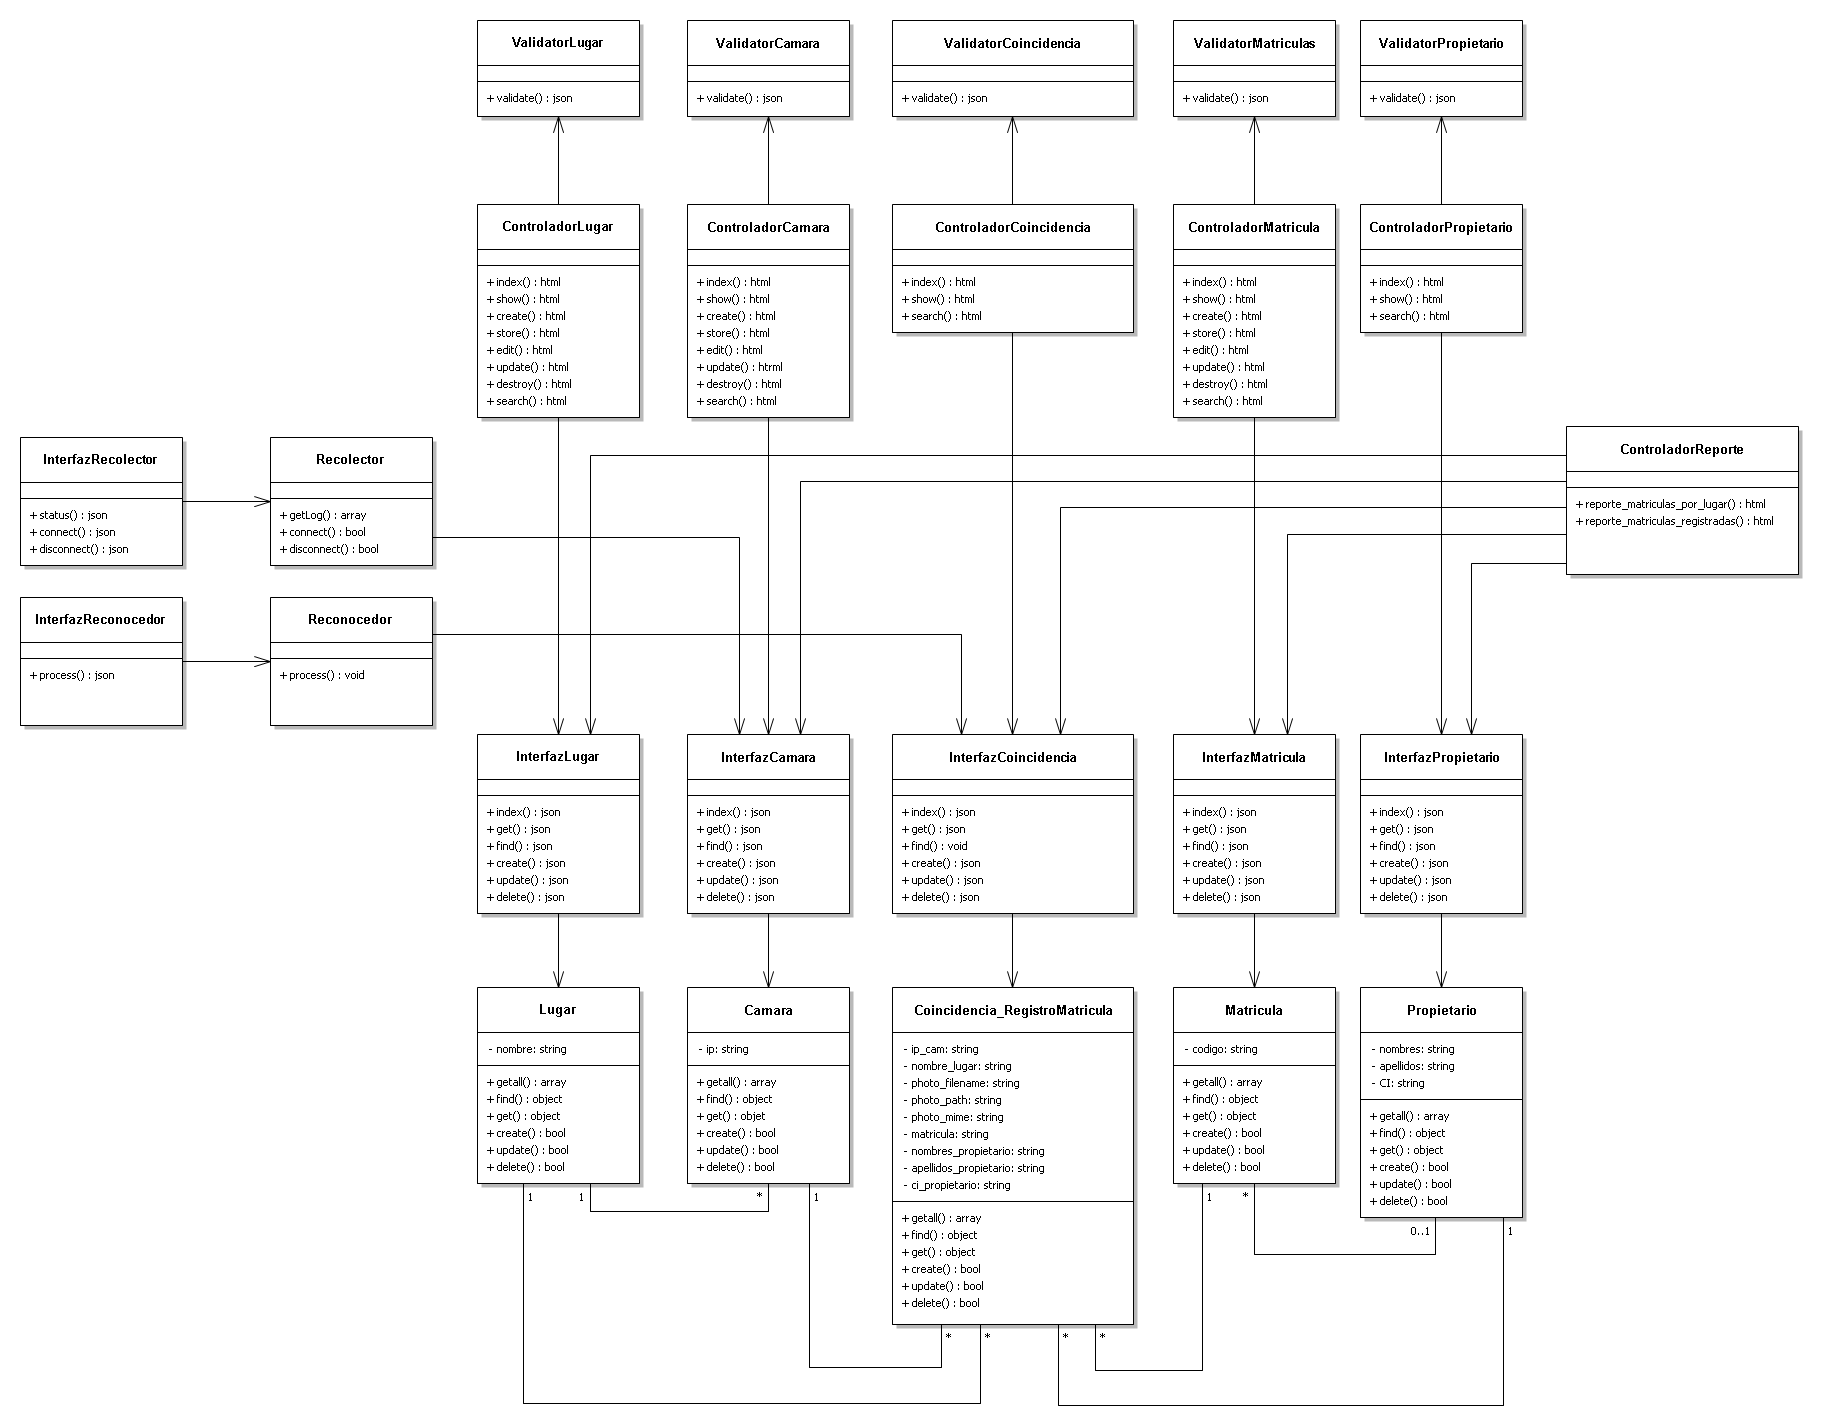
\includegraphics[width=1.2\textwidth]{CLASS}
%         \caption{Modelo Conceptual}
%         \label{fig:CLASS}
%     \end{figure}

% \newpage
% \eject \pdfpagewidth=215.9mm \pdfpageheight=279.4mm
 
\section{Modelo Físico}
    \begin{figure}[H]
        \centering
        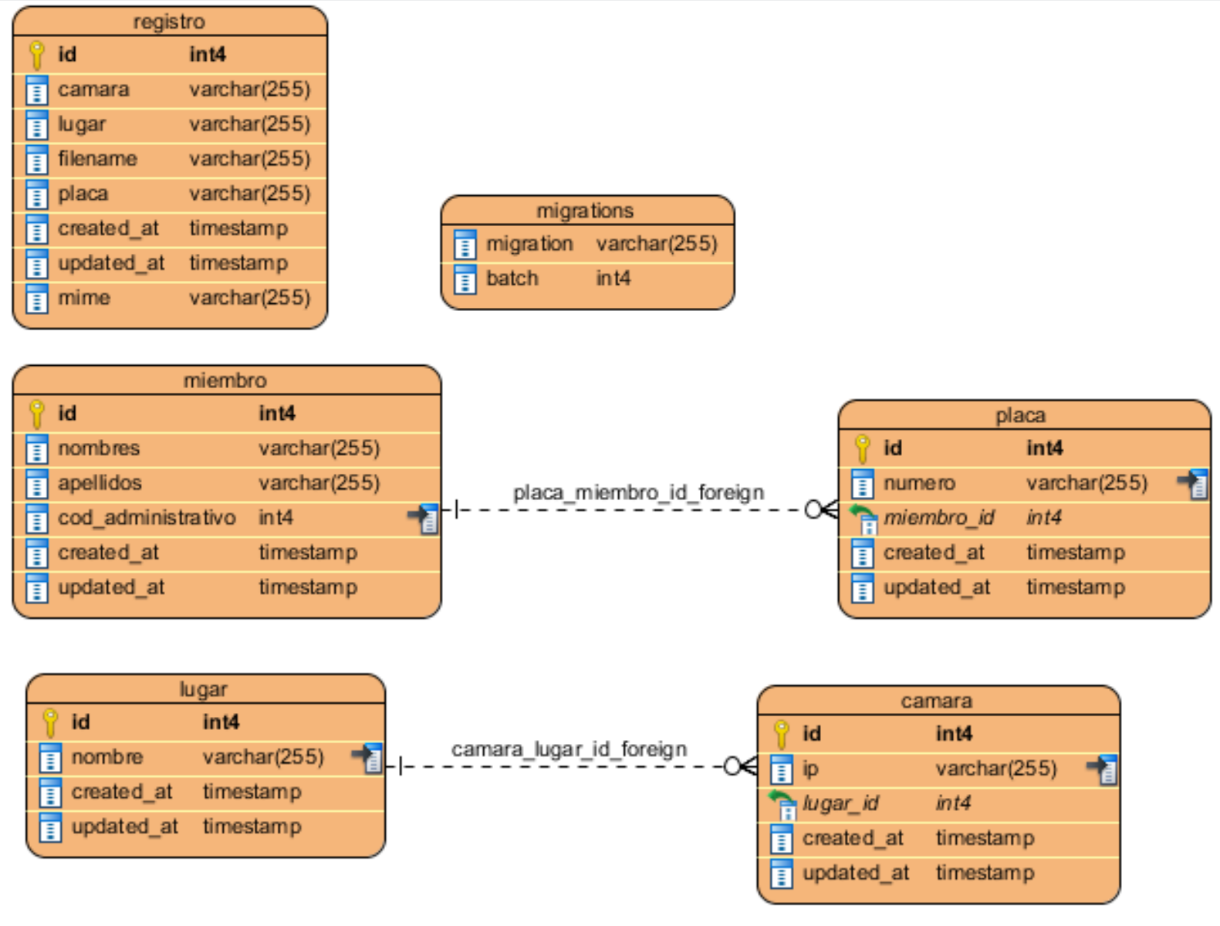
\includegraphics[width=.9\textwidth]{FISICO}
        \caption{Modelo Físico}
        \label{fig:FISICO}
    \end{figure}

\section{Estructura ICONIX para los Casos de Uso}
La descripción de cada caso de uso, de acuerdo con ICONIX, debe seguir la siguiente estructura: 
\begin{itemize}
    \item Descripción del Caso de Uso
    \item Diagrama de Caso de Uso
    \item Interfaz Gráfica Tentativa
    \item Diagrama de Robustez
    \item Diagrama de Secuencia
\end{itemize}
